
%(BEGIN_QUESTION)
% Copyright 2011, Tony R. Kuphaldt, released under the Creative Commons Attribution License (v 1.0)
% This means you may do almost anything with this work of mine, so long as you give me proper credit

Suppose the following control system is functioning as it is designed to, under regular operating conditions (i.e. stack temperature of 1550 $^{o}$F).  The metal temperature is holding perfectly at its setpoint value of 1425 $^{o}$F:

$$\includegraphics[width=15.5cm]{i03091x01.eps}$$

\noindent
Choose the best answer describing the immediate effect on this process if temperature transmitter TT-1 suddenly fails with a {\it high} signal:

\begin{itemize}
\item{} The furnace stack temperature will begin to rise as the controller calls for more heat
\vskip 10pt
\item{} The limiter relay (TY) will override the output signal from TIC-2
\vskip 10pt
\item{} The system will continue to operate normally, maintaining steady temperatures
\vskip 10pt
\item{} The valve will suddenly begin to close, decreasing heat input to the furnace
\end{itemize}

\underbar{file i03091}
%(END_QUESTION)





%(BEGIN_ANSWER)

The valve will suddenly begin to close, decreasing heat input to the furnace

%(END_ANSWER)





%(BEGIN_NOTES)

{\bf This question is intended for exams only and not worksheets!}.

%(END_NOTES)


